\onehalfspacing
\section{Đề số 26}

\begin{bt} 
   \begin{enumerate}[1)]
    \item Thực hiện phép tính
    \begin{enumerate}[a.]
        \item $\mathrm{A}=\frac{5}{15}+\frac{14}{25}-\frac{12}{9}+\frac{2}{7}+\frac{11}{25}$
        \item $B=\frac{2^{12} \cdot 3^5-4^6 \cdot 9^2}{\left(2^2 \cdot 3\right)^6+8^4 \cdot 3^5}-\frac{5^{10} \cdot 7^3-25^5 \cdot 49^2}{(125 \cdot 7)^3+5^9 \cdot 14^3}$
    \end{enumerate}
    \item Tìm $x, y, z$ biết:
    \begin{enumerate}[a.]
        \item $\left(3-\frac{9}{10}-|x+2|\right):\left(\frac{19}{10}-1-\frac{2}{5}\right)+\frac{4}{5}=1$ 
        \item $\frac{x}{3}=\frac{y}{4}, \frac{y}{3}=\frac{z}{5}$ và $2 x-3 y+z=6$
    \end{enumerate}
   \end{enumerate}
\loigiai{
    \begin{enumerate}[1)]
        \item \begin{enumerate}[a.]
            \item $A=\frac{5}{15}+\frac{14}{25}-\frac{12}{9}+\frac{2}{7}+\frac{11}{25} \\[5px]
            =\frac{-3}{3}+\frac{25}{25}+\frac{2}{7}=(-1+1)+\frac{2}{7}\\[5px] 
            =0+\frac{2}{7}=\frac{2}{7}$
            \item $B=\frac{2^{12} \cdot 3^5-2^{12} \cdot 3^4}{2^{12} \cdot 3^6+2^{12} \cdot 3^5}-\frac{5^{10} \cdot 7^3-5^{10} \cdot 7^4}{5^9 \cdot 7^3+5^9 \cdot 2^3 \cdot 7^3} \\[5px]
            = \frac{2^{12} \cdot 3^4 \cdot(3-1)}{2^{12} \cdot 3^5 \cdot(3+1)}-\frac{5^{10} \cdot 7^3 \cdot(1-7)}{5^9 \cdot 7^3 \cdot\left(1+2^3\right)} \\[5px]
            = \frac{2^{12} \cdot 3^4 \cdot 2}{2^{12} \cdot 3^5 \cdot 4}-\frac{5^{10} \cdot 7^3 \cdot(-6)}{5^9 \cdot 7^3 \cdot 9} \\[5px]
            = \frac{1}{6}-\frac{-10}{3}=\frac{7}{2}$
        \end{enumerate}
        \item \begin{enumerate}[a.]
            \item Ta có:\\[5px]
            $\left(3-\frac{9}{10}-|x+2|\right):\left(\frac{19}{10}-1-\frac{2}{5}\right)+\frac{4}{5}=1 \\[5px]
            \Leftrightarrow\left(\frac{30}{10}-\frac{9}{10}-|x+2|\right):\left(\frac{19}{10}-\frac{10}{10}-\frac{4}{10}\right)=1-\frac{4}{5} \\[5px]
            \Leftrightarrow\left(\frac{21}{10}-|x+2|\right): \frac{5}{10}=\frac{1}{5} \\[5px]
            \Leftrightarrow \frac{21}{10}-|x+2|=\frac{1}{5} \cdot \frac{5}{10}=\frac{1}{10} \\[5px]
            \Leftrightarrow|x+2|=\frac{21}{10}-\frac{1}{10}=2 \\[5px]
            \Leftrightarrow x+2=-2 ; 2 \\[5px]
            \Leftrightarrow x=-4 ; 0 \\[5px]
            \text {Vậy } x=0 ;-4$
            \item Từ giả thiết: $\frac{x}{3}=\frac{y}{4} \Rightarrow \frac{x}{9}=\frac{y}{12}$\\[5px]
            $\frac{y}{3}=\frac{z}{5} \Rightarrow \frac{y}{12}=\frac{z}{20}$\\[5px]
            Từ (1) và (2) suy ra: $\frac{x}{9}=\frac{y}{12}=\frac{z}{20}$\\[5px]
            Ta có: $\frac{x}{9}=\frac{y}{12}=\frac{z}{20}=\frac{2 x}{18}=\frac{3 y}{36}=\frac{z}{20}=\frac{2 x-3 y+z}{18-36+20}=\frac{6}{2}=3$\\[5px]
            Do đó: $\frac{x}{9}=3 \Rightarrow x=27$\\[5px]
            $\frac{y}{12}=3 \Rightarrow y=36 \\[5px]
            \frac{z}{20}=3 \Rightarrow z=60 \\[5px]
            \mathrm{KL}: x=27, y=36, z=60$
        \end{enumerate}
    \end{enumerate}
}
\end{bt}

\begin{bt}
    \hfill
	\begin{enumerate}[a.]
        \item Tìm x, y nguyên thoả mãn $3 x y-5=x^2+2 y$
        \item Chứng minh rằng với mọi số nguyên dương $\mathrm{n}$ thì: $3^{n+2}-2^{n+2}+3^n-2^n$ chia hết cho 10
    \end{enumerate}
	\loigiai{
        \begin{enumerate}
            \item Theo đề ta có $3 x y-2 y=x^2+5 \Rightarrow y(3 x-2)=x^2+5$\\[5px]
            Do $x, y$ nguyên nên suy ra $x^2+5$ chia hết cho $3 x-2$\\[5px]
            $\Rightarrow 9 .\left(x^2+5\right)$ chia hết cho $3 x-2$\\[5px]
            $\Rightarrow 9 \cdot x^2+45$ chia hết cho $3 x-2\\[5px] \Rightarrow 9 \cdot x^2-6 x+6 x-4+49$ chia hết cho $3 x-2$\\[5px]
            $\Rightarrow 3 x \cdot(3 x-2)+2(3 x-2)+49$ chia hết cho $3 x-2$\\[5px]
            $\Rightarrow 49$ chia hết cho $3 x-2 \Rightarrow 3 x-2 \in\{-49 ;-7 ;-1 ; 1 ; 7 ; 49\}$\\[5px]
            $\Rightarrow 3 x \in\{-47 ;-5 ; 1 ; 3 ; 9 ; 51\} \Rightarrow x \in\{1 ; 3 ; 17\}$\\[5px]
            Thay $x$ lần lượt vào (1) ta được $y \in\{6 ; 2 ; 6\}\\[5px] 
            $Vậy các cặp số $(x, y)$ là $(1 ; 6),(3 ; 2),(17 ; 6)$
            \item $3^{n+2}-2^{n+2}+3^n-2^n=\\[5px] 
            3^{n+2}+3^n-2^{n+2}-2^n \\[5px]
            =3^n\left(3^2+1\right)-2^n\left(2^2+1\right) \\[5px]
            =3^n \cdot 10-2^n \cdot 5=3^n \cdot 10-2^{n-1} \cdot 10 \\[5px]
            =10\left(3^n-2^{n-1}\right)$\\[5px]
            Vậy $3^{n+2}-2^{n+2}+3^n-2^n: 10$ với mọi $\mathrm{n}$ là số nguyên dương.
        \end{enumerate}
    } 
\end{bt}

\begin{bt}
    Cho đa thức: $\mathrm{A}(\mathrm{x})=\mathrm{x}+\mathrm{x}^2+\mathrm{x}^3+\ldots+\mathrm{x}^{99}+\mathrm{x}^{100}$.
    \begin{enumerate}[a.]
        \item Chứng minh rằng $x=-1$ là nghiệm của $\mathrm{A}(\mathrm{x})$
        \item Tính giá trị biểu thức $\mathrm{A}(\mathrm{x})$ khi $\mathrm{x}=\frac{1}{2}$
    \end{enumerate}
	\loigiai{
        \begin{enumerate}
            \item $A(-1)=(-1)+(-1)^2+(-1)^3+\ldots+(-1)^{99}+(-1)^{100} \\[5px]
            =-1+1+(-1)+1+(-1)+\ldots(-1)+1=0$ (vì có 50 số -1 và 50 số 1 )\\[5px]
            Suy ra $\mathrm{x}=-1$ là nghiệm của đa thức $\mathrm{A}(\mathrm{x})$\\[5px]
            \item $\text {Với } x=\frac{1}{2} \text { thì giá trị của đa thức } \mathrm{A}=\frac{1}{2}+\frac{1}{2^2}+\frac{1}{2^3}+\ldots+\frac{1}{2^{98}}+\frac{1}{2^{99}}+\frac{1}{2^{100}} \\[5px]
            \Rightarrow 2A=2\left(\frac{1}{2}+\frac{1}{2^2}+\frac{1}{2^3}+\ldots+\frac{1}{2^{98}}+\frac{1}{2^{99}}+\frac{1}{2^{100}}\right)=1+\frac{1}{2}+\frac{1}{2^2}+\frac{1}{2^3}+\ldots+\frac{1}{2^{98}}+\frac{1}{2^{99}} \\[5px]
            \Rightarrow 2 \mathrm{~A}=\left(\frac{1}{2}+\frac{1}{2^2}+\frac{1}{2^3}+\ldots+\frac{1}{2^{98}}+\frac{1}{2^{99}}+\frac{1}{2^{100}}\right)+1-\frac{1}{2^{100}} \Rightarrow 2 A=A+1-\frac{1}{2^{100}} \\[5px]
            \Rightarrow A=1-\frac{1}{2^{100}}$
        \end{enumerate}
    }
\end{bt}

\begin{bt}
    Cho $\triangle A B C(\mathrm{AB}>\mathrm{AC}), \mathrm{M}$ là trung điểm của $\mathrm{BC}$. Đường thẳng đi qua $\mathrm{M}$ vuông góc với tia phân giác của góc $B A C$ cắt cạnh $\mathrm{AB}, \mathrm{AC}$ lần lượt tại $\mathrm{E}$ và $\mathrm{F}$ (giao điểm của đường thẳng đó với tia phân giác góc $BAC$ là $H$ ). Chứng minh rằng:
    \begin{enumerate}[a.]
        \item $\mathrm{EH}=\mathrm{HF}$
        \item $2 \mathrm{BME}=\mathrm{ACB}-\mathrm{B}$.
        \item $\frac{F E^2}{4}+A H^2=A E^2$.
        \item $\mathrm{BE}=\mathrm{CF}$
    \end{enumerate}
	\loigiai{
        $$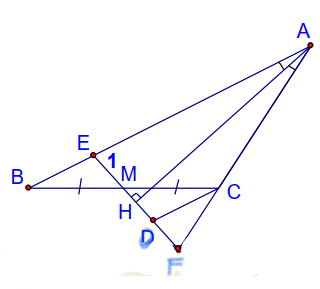
\includegraphics[width=0.4\textwidth]{26-4-lg.png}$$
        \begin{enumerate}
            \item $\mathrm{C} / \mathrm{m}$ được $\triangle A E H=\triangle A F H$ (g-c-g) Suy ra $\mathrm{EH}=\mathrm{HF}$ (đpcm)
            \item Từ $\triangle A E H=\triangle A F H$ Suy ra $E_1=F$\\[5px]
            Xét $\triangle C M F$ có $A C B$ là góc ngoài suy ra $C M F=A C B-F$\\[5px] 
            $\triangle B M E$ có $E_1$ là góc ngoài suy ra $B M E=E_1-B$\\[5px]
            Vậy $C M F+B M E=(A C B-F)+\left(E_1-B\right)$
            hay $2 B M E=A C B-B($ đpcm $)$.
            \item Áp dụng định lí Pytago vào tam giác vuông $\mathrm{AFH}$ :\\[5px]
            ta có $\mathrm{HF}^2+\mathrm{HA}^2=\mathrm{AF}^2$ hay $\frac{F E^2}{4}+A H^2=A E^2$ (đpcm)
            \item $\mathrm{C} / \mathrm{m} \triangle A H E=\triangle A H F(g-c-g)$ Suy ra $\mathrm{AE}=\mathrm{AF}$ và $E_1=F$\\[5px]
            Từ $C$ vẽ $C D / / A B(D \in E F)$\\[5px]
            $\mathrm{C} / \mathrm{m}$ được $\triangle B M E=\triangle C M D(g-c-g) \Rightarrow B E=C D$\\[5px]
            Và có $E_1=C D F$ (cặp góc đồng vị)\\[5px]
            Do đó $C D F=F \quad \Rightarrow \quad \Delta C D F$ cân $\Rightarrow C F=C D$\\[5px]
            Từ (1) và (2) suy ra $B E=C F$
        \end{enumerate}
    }
\end{bt}

\begin{bt}
   Giải bằng máy tính cầm tay:
   \begin{enumerate}[a.]
    \item Tính giá trị của đa thức $\mathrm{P}(\mathrm{x})=1+\mathrm{x}+\mathrm{x}^2+\mathrm{x}^3+\ldots .+\mathrm{x}^{10}$ tại $\mathrm{x}=2,13$ (kết quả ghi dưới dạng số thập phân lấy trên màn hình).
    \item Tìm 2 chữ số cuối của: $A=2^{2010}+2^{2011}+2^{2012}+2^{2013}+2^{2014}+2^{2015}+2^{2016}$
   \end{enumerate}
\loigiai{
    \begin{enumerate}
        \item Cách 1: Ta có thức $P(x)=1+x+x^2+x^3+\ldots .+x^{10}=\frac{x^{11}-1}{x-1}$\\[5px]
        Thay $x=2,13$ ta được kết quả $P(2,13)=\frac{2,13^{11}-1}{2,13-1} \approx 3622,355813$.\\[5px]
        Cách 2: Nhập vào máy: $\sum_{\mathrm{x}=0}^{10}\left(2,13^{\mathrm{x}}\right) \boxminus$ ta được kết quả $\mathrm{P}(2,13) \approx 3622,355813$.
        \item $\mathrm{HD}$ :\\[5px]
        $A=2^{2000}\left(2^{10}+2^{11}+2^{12}+2^{13}+2^{14}+2^{15}+2^{16}\right) \\[5px]
        =\left(2^{20}\right)^{100} \times 130048 \\[5px]
        \text {mà } 2^{20}=\left(2^{10}\right)^2=1024^2=1048576$\\[5px]
        Ta nhận thấy bất kỳ một số có đuôi là 76 thì lũy thừa luôn luôn có đuôi là 76 (dùng máy để kiểm tra)\\[5px]
        Do đó: $\mathrm{A}=130048 \times(\ldots 76)=\ldots .48$. Vậy 2 số cuối của $\mathrm{A}$ có giá trị là 48
    \end{enumerate}
}
\end{bt}


